%TC:group table 0 1
%TC:group tabular 1 1

\chapter{Implementation}

This chapter gives an overview of the implementation of the project, discussing the implementation and optimisation of the core Prolog interpreter (Section \ref{sec:core-interpreter}), its garbage collector (Section \ref{sec:gc-impl}), the JavaScript foreign function interface (Section \ref{sec:js-ffi}), and the web-based development environment (Section \ref{sec:web-dev-env}).

\section{Repository Overview}

\begin{table}[H]
\centering
\begin{tabular}{lp{9cm}l}
\hline
\textbf{Directory} & \textbf{Description} & \textbf{LOC} \\
\hline
\texttt{core/} & Implementation of the core interpreter in Rust, including the parser, garbage collector, and the JavaScript FFI. & 2664 (Rust) \\
\texttt{core/src/wasm} & WebAssembly interface for the core interpreter and JavaScript FFI. & \\
\texttt{core/src/tests} & Unit tests for the core interpreter. & \\
\texttt{lib/} & Higher-level JavaScript library for the interpreter. & 81 (JS) \\
\texttt{web/} & Web-based development environment to demonstrate and benchmark the interpreter. & 836 (TS) \\
\texttt{web/src/prolog} & TypeScript Prolog interface and wrappers for various Prolog interpreters. & \\
\texttt{bench/} & Web-based benchmarking tools. & 165 (JS \& Python) \\
\texttt{docs/} & Documentation for the project. & N/A \\
\hline
& \hfill \textbf{Total} & \textbf{3746} \\
\hline
\end{tabular}
\caption{An overview of key directories in the repository}
\label{tab:repository-overview}
\end{table}

\section{Core Interpreter}

\label{sec:core-interpreter}

This section describes the implementation of the core Prolog interpreter, WebPL, implemented in Rust.

\subsection{Memory Layout}

\label{sec:memory-layout}

WebPL uses the merged heap/stack architecture proposed by Li \cite{liEfficientMemoryManagement2000} and described in Section \ref{sec:preparation-implementation}. Alongside the advantages identified by Li, notably improved cache performance, this architecture is uniquely suited to the linear memory model of WebAssembly.

In a traditional heap/stack architecture, the heap and stack are separate regions of memory, often with few constraints imposed on the heap layout. Indeed, SWI-Prolog uses \texttt{malloc} to allocate memory for terms on the heap\footnote{\url{https://www.swi-prolog.org/pldoc/man?section=memlimit}}, imposing no constraints on its layout. Running natively, this is not a problem, as virtual memory is plentiful. However, WebAssembly's linear memory is contiguous, so the heap must be carefully managed by the WebAssembly code itself to avoid fragmentation. In addition, the trail stack contains pointers to bound variables, which may appear either on the stack or on the heap, but WebAssembly does not allow pointers to stack-allocated objects (Section \ref{sec:wasm-memory-model}). Therefore, the stack must also be placed in the linear memory, further complicating memory management.

In a merged heap/stack architecture, all terms are allocated in one contiguous region of memory. This avoids the problem of fragmentation, as the heap grows with allocations and shrinks with instant reclaiming and garbage collection (Section \ref{sec:gc-impl}). If the heap grows too large for the linear memory, it suffices to execute the \texttt{memory.grow} WebAssembly instruction, with minimal additional work from the WebAssembly module required.

A key advantage of this architecture is that the heap is stored in chronological order, with older terms at lower addresses. This facilitates the implementation of several garbage collection optimisations, such as variable shunting (Section \ref{sec:variable-shunting}) and segmented garbage collection (Section \ref{sec:implementation-generational-gc}).

Of course, other areas of memory are needed, also within the linear memory:

\paragraph{Trail Stack} The trail stack is a stack of pointers to variables that have been bound, used for backtracking.

\paragraph{Choice-Point Stack} The choice-point stack stores information about where to backtrack to for each choice we make. Alongside the next clause to consider, each choice point also contains the sizes of the heap, trail stack and goal stack to facilitate backtracking and instant reclaiming (Section \ref{sec:prolog-gc}).

\paragraph{Goal Stack} The goal stack contains the remaining goals to prove. When backtracking, goals that have previously been popped might be needed again, so while I refer to it as a stack, the goal stack is actually a graph, with goals represented as pairs $(\texttt{pred}, \texttt{goal})$ and the goal stack additionally storing a pointer to the current goal (the ``top of the stack'').

Figure \ref{fig:goals} illustrates this idea. Before resolving \mintinline{prolog}{a(X)} with \mintinline{prolog}{a(1)} (c), a choice point is created, containing a pointer to the current goal. After the resolution step, \mintinline{prolog}{a(X)} is ``popped from the goal stack'' by setting the current goal pointer to its predecessor (d). Importantly, however, it remains in the graph, as upon backtracking when \mintinline{prolog}{b(1)} fails, the current goal pointer is restored to that stored in the choice point. In order to prevent the goal stack growing indefinitely, each choice point also contains the number of goals in the stack when it was created, and the goal stack is truncated to this size upon backtracking.

\begin{figure}[H]
\centering
\begin{subfigure}{.5\textwidth}
\centering
\begin{minted}{prolog}
a(1).
a(2).
b(2).
?- a(X), b(X).

\end{minted}
\caption{A Prolog program}
\end{subfigure}%
\begin{subfigure}{.5\textwidth}
\centering
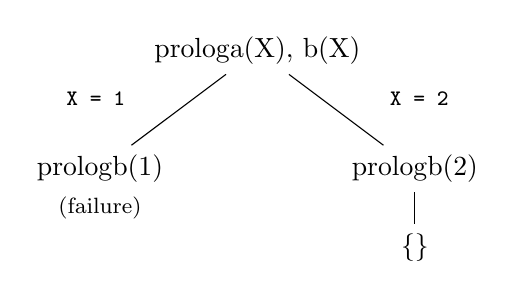
\begin{tikzpicture}
  \node (A) at (0,3) {\mintinline{prolog}{a(X), b(X)}};
  \node (B1) at (-2,1.5) {\mintinline{prolog}{b(1)}};
  \node (B2) at (2,1.5) {\mintinline{prolog}{b(2)}};
  \node (C2) at (2,0.5) {\{\}};

  \draw (A) -- (B1) node [midway, xshift=-30, yshift=4] {\footnotesize \texttt{X = 1}};
  \draw (A) -- (B2) node [midway, xshift=30, yshift=4] {\footnotesize \texttt{X = 2}};
  \draw (B2) -- (C2);

  \node (D) at (-2,1) {\footnotesize (failure)};
\end{tikzpicture}
\caption{Corresponding SLD-tree}
\end{subfigure}
\par\bigskip
\par\bigskip
\begin{subfigure}{.5\textwidth}
\centering
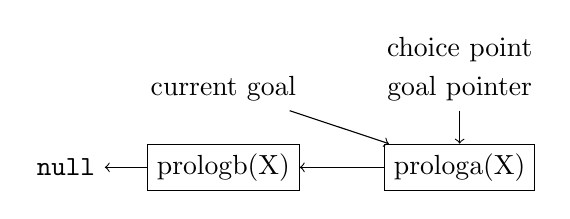
\begin{tikzpicture}[box/.style={draw, rectangle}]
  \node[box] (B) at (0, 0) {\mintinline{prolog}{b(X)}};
  \node[box] (A) at (3, 0) {\mintinline{prolog}{a(X)}};

  \node (null) at (-2, 0) {\texttt{null}};
  \node (current) at (0, 1) {current goal};
  \node (cp1) at (3, 1.5) {choice point};
  \node (cp2) at (3, 1) {goal pointer};

  \draw[->] (A) -- (B);
  \draw[->] (B) -- (null);
  \draw[->] (current) -- (A);
  \draw[->] (cp2) -- (A);
\end{tikzpicture}
\vspace{5mm}
\caption{The goal graph before the first resolution}
\end{subfigure}%
\begin{subfigure}{.5\textwidth}
\centering
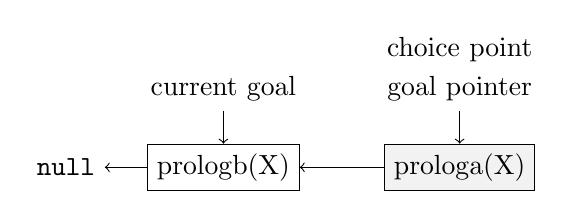
\begin{tikzpicture}[box/.style={draw, rectangle}]
  \node[box] (B) at (0, 0) {\mintinline{prolog}{b(X)}};
  \node[box, fill=black!5] (A) at (3, 0) {\mintinline{prolog}{a(X)}};

  \node (null) at (-2, 0) {\texttt{null}};
  \node (current) at (0, 1) {current goal};
  \node (cp1) at (3, 1.5) {choice point};
  \node (cp2) at (3, 1) {goal pointer};

  \draw[->] (A) -- (B);
  \draw[->] (B) -- (null);
  \draw[->] (current) -- (B);
  \draw[->] (cp2) -- (A);
\end{tikzpicture}
\vspace{5mm}
\caption{The goal graph after the first resolution}
\end{subfigure}
\vspace*{-5mm}
\caption{The goal graph}
\label{fig:goals}
\end{figure}

To avoid the need to garbage collect the goal stack, goals are removed from the graph when they are popped if they are not reachable from any choice points (Section \ref{sec:choice-point-elimination}).

\paragraph{Code Area} There is no separate code area, as the clauses of the program are stored on the heap using the same representation as ordinary terms, an idea proposed by Tarau for his ``hitchhiker'' Prolog implementation \cite{tarauHitchhikersGuideReinventing2018}. Initially, my implementation used a distinct code area, but profiling revealed that up to 40\% of the execution time was spent copying terms onto the heap. Benchmarking confirmed that Tarau's approach reduced mean execution time by around 25\%.

Following this approach, copying a clause onto the heap when a goal unifies with its head consists of a single \texttt{memcpy} followed by a linear scan of the copied clause terms to add the appropriate offset to any pointers. To efficiently identify the byte boundaries between terms in the body of the clause, each clause additionally includes a header containing $n$ variables, bound to the $n$ terms in its body (Figure \ref{fig:clause-layout}).

\begin{figure}[H]
\centering
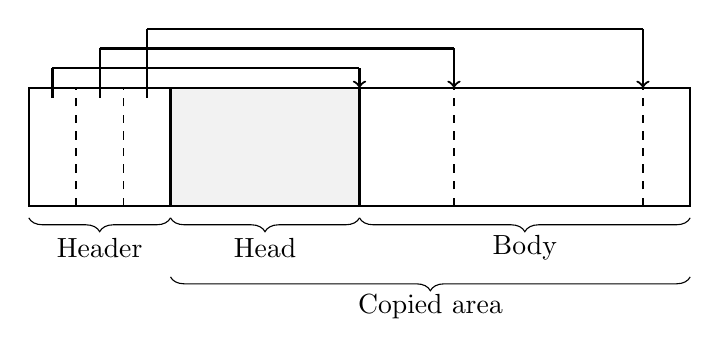
\begin{tikzpicture}[xscale=1.2,yscale=0.5]

\fill[thick, black!5] (2,0) rectangle (4,3);
\draw[thick] (0.5,0) rectangle (7.5,3);

\draw[thick] (2,0) -- (2,3);
\draw[thick] (4,0) -- (4,3);

\foreach \x in {1, 1.5, 5, 7} {
    \draw[dashed] (\x,0) -- (\x,3);
}

\draw[thick] (0.75,2.75) -- (0.75,3.5);
\draw[thick] (0.75,3.5) -- (4,3.5);
\draw[->, thick] (4,3.5) -- (4,3);

\draw[thick] (1.25,2.75) -- (1.25,4);
\draw[thick] (1.25,4) -- (5,4);
\draw[->, thick] (5,4) -- (5,3);

\draw[thick] (1.75,2.75) -- (1.75,4.5);
\draw[thick] (1.75,4.5) -- (7,4.5);
\draw[->, thick] (7,4.5) -- (7,3);

\draw [decorate,decoration={brace,amplitude=5pt,mirror,raise=1ex}] (0.5,0) -- (2,0) node[midway,yshift=-1.5em]{Header};
\draw [decorate,decoration={brace,amplitude=5pt,mirror,raise=1ex}] (2,0) -- (4,0) node[midway,yshift=-1.5em]{Head};
\draw [decorate,decoration={brace,amplitude=5pt,mirror,raise=1ex}] (4,0) -- (7.5,0) node[midway,yshift=-1.5em]{Body};

\draw [decorate,decoration={brace,amplitude=5pt,mirror,raise=1ex}] (2,-1.5) -- (7.5,-1.5) node[midway,yshift=-1.5em]{Copied area};

\end{tikzpicture}
\caption{Memory layout of a clause on the heap}
\label{fig:clause-layout}
\end{figure}

\vspace*{-2em}

\paragraph{Lambda Table} Each lambda term (Section \ref{sec:term-representation}) contains an index into the \emph{lambda table}. This contains an entry for each lambda term in the program source, which comprises the JavaScript code and the names it uses to refer to its arguments (Section \ref{sec:js-ffi}).

\subsection{Pointers}

\label{sec:pointers}

A common theme in my implementation, taken from WebAssembly, is that of preferring indexing over pointers. The contiguous nature of the heap allows terms to be referred to by their index, and the same is true for the goal and choice-point stacks.

Rust discourages the use of raw pointers, instead preferring its memory-safe \emph{references}. Every object in Rust has exactly one \emph{owner}, with multiple immutable references or a single mutable reference allowed, enforced at compile time by the \emph{borrow checker}. The Prolog heap does not fit nicely into this model: multiple variables may be bound to the same term, all requiring mutable access to it (e.g. to update the term when unifying). One way to work around this is to use reference counting and \texttt{RefCell}, which facilitates runtime borrow checking, but this is very slow. Instead, terms are referred to by their index in the heap (although this may be informally referred to as a ``pointer''). The merged heap/stack architecture makes this straightforward to implement.

\subsection{Term Representation}

\label{sec:term-representation}

Terms are stored on the heap as fixed-size blocks of 16 bytes. These are represented as an enum (Figure \ref{fig:rust-term-representation}), Rust's sum type.

Atoms are typed, being strings, integers, or floats. Variables include a pointer to their bound object if they are bound, or to themselves otherwise, as in the WAM, but additionally a flag to indicate whether they are \emph{shunted} (Section \ref{sec:variable-shunting}), which is used in garbage collection, and possibly a pointer to a \emph{suspended goal} (Section \ref{sec:attributed-variables}). Compound terms, represented by their functor and arity $n$, are followed in the heap by $n$ variables pointing to each of their arguments (Figure \ref{fig:compound}). This allows their variable-sized arguments to be found in constant time, while keeping their layout contiguous. There is also a heap representation of cut, as goals are stored on the heap. Finally, \emph{lambda terms}, used to call JavaScript code from within Prolog (Section \ref{sec:js-ffi}), are represented by an index into the \emph{lambda table}, along with their arguments like a compound term.

\begin{figure}[H]
\centering
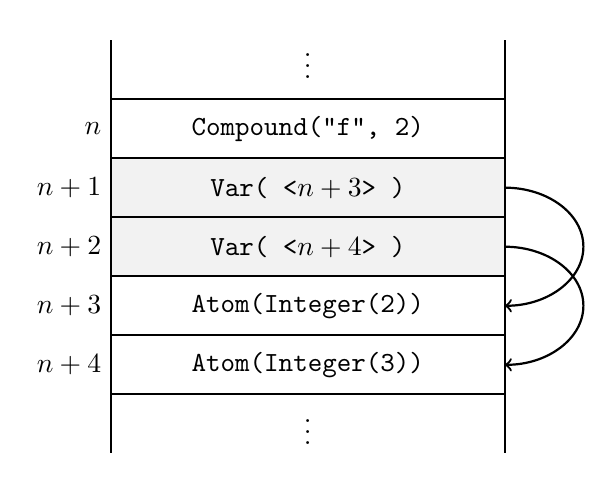
\begin{tikzpicture}[yscale=0.75]
    \node at (2.5,0.7) {\vdots};
        \fill[thick,black!5] (0,-3) rectangle (5,-1);

        \draw[thick] (0,1) -- (0,-6);
        \draw[thick] (5,1) -- (5,-6);
        \draw[thick] (0,0) rectangle (5,-1);
        \draw[thick] (0,-1) rectangle (5,-2);
        \draw[thick] (0,-2) rectangle (5,-3);
        \draw[thick] (0,-3) rectangle (5,-4);
        \draw[thick] (0,-4) rectangle (5,-5);
        \node at (2.5,-5.5) {\vdots};
        \node at (2.5,-0.5) {\texttt{Compound("f", 2)}};
        \node at (2.5,-1.5) {\texttt{Var( <$n+3$> )}};
        \node at (2.5,-2.5) {\texttt{Var( <$n+4$> )}};
        \node at (2.5,-3.5) {\texttt{Atom(Integer(2))}};
        \node at (2.5,-4.5) {\texttt{Atom(Integer(3))}};
        \draw[->, thick] (5,-1.5) arc[start angle=90, end angle=-90, radius=1];
        \draw[->, thick] (5,-2.5) arc[start angle=90, end angle=-90, radius=1];

        \node[anchor=east] at (0,-0.5) {$n$};
        \node[anchor=east] at (0,-1.5) {$n+1$};
        \node[anchor=east] at (0,-2.5) {$n+2$};
        \node[anchor=east] at (0,-3.5) {$n+3$};
        \node[anchor=east] at (0,-4.5) {$n+4$};
\end{tikzpicture}
\caption{Heap representation of \texttt{f(2, 3)}}
\label{fig:compound}
\end{figure}

\vspace*{-1.5em}

All other kinds of term supported in the syntax are syntactic sugar for terms represented as above, converted during parsing. For example, the arithmetic expression $2 + 3$ becomes the compound term \texttt{+(2, 3)}, and the list \texttt{[a, b]} becomes the compound term \texttt{.(a, .(b, []))}.

\begin{figure}[H]
\centering
\begin{subfigure}{0.7\textwidth}
\centering
\begin{minted}{rust}
pub enum HeapTerm {
    Atom(Atom),
    Var(HeapTermPtr, bool, bool, HeapTermPtr),
    Compound(StringId, usize), // followed by args
    Cut(ChoicePointIdx),
    Lambda(LambdaId, usize), // followed by args
}
\end{minted}
\end{subfigure}%
\begin{subfigure}{0.3\textwidth}
\centering
\begin{minted}{rust}
pub enum Atom {
    String(StringId),
    Integer(i64),
    Float(f64),
}


\end{minted}
\end{subfigure}
\caption{Term representation in Rust}
\label{fig:rust-term-representation}
\end{figure}

\subsection{Parsing}

The Prolog program is parsed into its abstract syntax tree using a parser generated by LALRPOP \cite{thelalrpopprojectdevelopersLALRPOPhttpsgithubcom2015} with a custom grammar.

\begin{figure}[H]
\centering
\begin{minted}{rust}
Clause: Clause = {
    <h:Term> "." => Clause(h, vec![]),
    <h:Term> ":-" <b:Comma<Term>> "." => Clause(h, b),
}
Comma<T>: Vec<T> = {
    <t:T> => vec![t],
    <mut ts:Comma<T>> "," <t:T> => { ts.push(t); ts },
}
\end{minted}
\caption{Extract from the LALRPOP grammar}
\label{fig:grammar}
\end{figure}

\vspace*{-1.5em}

Figure \ref{fig:grammar} shows the definition of \texttt{Clause} and \texttt{Comma<T>} in the grammar. LALRPOP supports polymorphic non-terminals, which are used to define a generic non-empty comma-separated list of terms, \texttt{Comma<T>}.

\subsection{Built-in Predicates}

\label{sec:builtins}

To perform useful computation, the interpreter must support some built-in predicates, such as arithmetic evaluation. The full set of built-in predicates is given in Appendix \ref{appendix:predicates}.

Each predicate implements a Rust \emph{trait}, similar to an interface in C++, called \texttt{Builtin} (Figure \ref{fig:builtin-trait}). This trait has an associated constant, \texttt{ARITY}, the number of arguments the predicate takes. The \texttt{eval} function takes a pointer to the first argument and evaluates the predicate, potentially modifying the interpreter state through the mutable \texttt{Solver} reference, returning a boolean if the predicate succeeded or failed with no errors, or returning an error of type \texttt{BuiltinError}, for example if an argument was insufficiently instantiated.

\begin{figure}[H]
\centering
\begin{minted}{rust}
pub trait Builtin<const ARITY: usize> {
    fn eval(solver: &mut Solver, args: HeapTermPtr)
        -> Result<bool, BuiltinError>;
}
\end{minted}
\caption{The \texttt{Builtin} trait}
\label{fig:builtin-trait}
\end{figure}

Many built-in predicates are implemented near-identically, for example the extra-logical type-testing predicates \texttt{var/1} and \texttt{atom/1}, which only differ in the type they compare against. To avoid code duplication, these predicates are implemented using meta-programming, with a \emph{macro} generating the code for each type (Figure \ref{fig:builtin-macro}). It uses Rust's pattern-matching syntax to match the term's heap representation against a pattern \texttt{\$matcher}.

\begin{figure}[H]
\centering
%TC:ignore
\begin{minted}{rust}
macro_rules! impl_type_check {
    ($name:ident, $matcher:pat) => {
        pub struct $name;
        impl Builtin<1> for $name {
            fn eval(solver: &mut Solver, args: HeapTermPtr)
                -> Result<bool, BuiltinError>
            {
                Ok(matches!(solver.heap.get(args), $matcher))
            }
        }
    };
}

impl_type_check!(IsAtomBuiltin, HeapTerm::Atom(_));
impl_type_check!(IsVarBuiltin, HeapTerm::Var(_, _, _, _));
\end{minted}
%TC:endignore
\caption{Macro for type-testing predicates}
\label{fig:builtin-macro}
\end{figure}

\subsection{Cut}

The cut operator, \texttt{!/0}, is an extra-logical predicate that commits to the clause in which it appears. In other words, backtracking past a cut causes the predicate it appears in to fail.

When a clause is copied onto the heap, a linear scan updates its variables by the appropriate offset (Section \ref{sec:memory-layout}). This also updates any instances of the cut operator to include the index of the current choice point, that is, the one before this clause was selected. When the cut operator becomes the current goal and is executed, the choice-point stack is truncated to the choice point referred to by the cut.

\subsection{Attributed Variables}

\label{sec:attributed-variables}

Like many Prolog implementations, WebPL includes some features from constraint logic programming. \emph{Attributed variables}, or \emph{suspensions}, allow a term to be attached to a variable, which is executed when the variable is bound \cite{holzbaurMetastructuresvsattributed1992}. This allows constraints to be attached to variables and checked later when more information is available. Two common uses of attributed variables are in the \texttt{freeze/2} and \texttt{dif/2} predicates, the former delaying the execution of a goal until a variable is bound to a non-variable term, and the latter ensuring that two variables, when bound, cannot be unified.

I implemented a basic form of attributed variables, where attributes are limited to goals, as described by Carlsson \cite{carlssonimplementationdiffreeze1986}. A \texttt{delay/2} built-in predicate is used as the basis for this implementation, which takes a term and a goal as arguments. If the term is not yet bound, the goal becomes the term's \emph{suspended goal} in its heap representation, otherwise it is immediately pushed to the goal stack (Figure \ref{fig:delay-impl}). The predicate succeeds in either case. When an attributed variable is bound, its suspended goal is pushed to the goal stack and removed from its heap representation.

\begin{figure}[H]
\centering
\begin{minted}{rust}
match &mut solver.heap.data[var] {
    HeapTerm::Var(_, _, has_attr, attr) => {
        *has_attr = true;
        *attr = goal;
    }
    _ => solver.goals.push(goal),
}
\end{minted}
\caption{Implementation of \texttt{delay/2}}
\label{fig:delay-impl}
\end{figure}

While \texttt{delay/2} is sufficient to implement both \texttt{freeze/2} and \texttt{dif/2}, I implemented \texttt{freeze/2} directly as a built-in predicate to improve performance. The implementation of this predicate is identical to that of \texttt{delay/2}, except that it attaches the current goal (i.e. \texttt{freeze(..., ...)}) to the variable to account for intermediate unifications to variable terms.

\subsection{Choice-Point Elimination (incl. Last-Call Optimisation)}

\label{sec:choice-point-elimination}

Last-call optimisation (LCO) is traditionally implemented by reusing the stack frame for the last call of a determinate predicate (Section \ref{sec:preparation-implementation}). This is applicable on the final clause of a predicate, or after a cut.

However, WebPL does not have a call stack, instead storing all terms on the heap and using a goal stack and choice-point stack for control (Section \ref{sec:memory-layout}). Therefore, LCO must be implemented in two parts, one on the choice-point stack and one on the goal stack.

For the choice-point stack, I do not create a choice point for the final clause of a predicate, as its failure necessarily implies the failure of the entire predicate, which I call \emph{choice-point elimination}. Static analysis prior to execution is performed to group clauses into predicates to enable this. This has the same effect as traditional LCO: if a clause is determinate, it will not leave any choice points on the stack, as no choice point will be created for either the choice of the clause or the solution of any goals. In the case where a clause cannot be reached because of a cut, this is also sound, as the cut will remove any choice points created by the clause.

Recall the implementation of the goal stack from Section \ref{sec:memory-layout}, namely that ``popping a goal from the stack'' does not remove it from the graph, rather moving the current goal pointer to its predecessor. If goals are only fully removed on backtracking, when the goal stack is truncated, a determinate predicate will use linear space on the goal stack, despite using constant space on the choice-point stack.

However, when no choice points refer to a goal, it is sound to remove it from the graph entirely when it is popped. This is exactly the case in a determinate predicate. The goals of its body are pushed to the goal stack when a goal unifies with its head, and because of its determinacy and choice-point elimination, no choice points are created as these goals are popped and resolved one by one. Furthermore, as they will be allocated at the end of the memory for the goal graph, no fragmentation occurs when they are removed. This is implemented by passing a flag to \texttt{Goal::pop}, indicating whether the goal can be safely removed (Figure \ref{fig:goal-pop}).

\begin{figure}[H]
\centering
\begin{minted}{rust}
impl Goal {
    pub fn pop(&mut self, determinate: bool) {
        if let Some(ptr) = self.current.take() {
            self.current = self.goals[ptr].prev_ptr();
            if determinate && ptr == self.goals.len() - 1 {
                self.goals.pop();
            }
        }
    }
}
\end{minted}
\caption{Implementation of \texttt{Goal::pop}}
\label{fig:goal-pop}
\end{figure}

\subsection{String Interning}

Strings are expensive to copy because they must be dynamically allocated in the linear memory. Comparing two strings of length $n$ for equality is also far more expensive than an arithmetic comparison, requiring both loads and $O(n)$ comparisons, as opposed to a single WebAssembly instruction for arithmetic comparison.

For this reason, WebPL avoids using \texttt{String} objects wherever possible by using \emph{string interning}. Strings are allocated in a specific area of memory, and references to each string are replaced with its index in that area. A hash table, mapping strings to their indices, prevents duplicates.

A further optimisation initialises the string area with fixed mappings for commonly-used strings, like the names of built-in predicates and arithmetic operators. For example, the string \texttt{"+"} is always at index 9, stored as a Rust constant \texttt{str::ADD}, so a real string comparison is not necessary, even with runtime-generated strings (due to the uniqueness of string mapping). Figure \ref{fig:fixed-string-indices} shows how this optimises the arithmetic evaluation code (simplified).

\begin{figure}[H]
\centering
\begin{subfigure}{.5\textwidth}
\centering
\begin{minted}{rust}
match functor {
    str::ADD /*  9 */ => add(&a, &b),
    str::SUB /* 10 */ => sub(&a, &b),
    str::MUL /* 11 */ => mul(&a, &b),
    str::DIV /* 12 */ => div(&a, &b),
    ...
}
\end{minted}
\caption{Arithmetic comparison of functors}
\end{subfigure}%
\begin{subfigure}{.5\textwidth}
\centering
\begin{minted}{rust}
match lookup_string(functor) {
    "+" => add(&a, &b),
    "-" => sub(&a, &b),
    "*" => mul(&a, &b),
    "/" => div(&a, &b),
    ...
}
\end{minted}
\caption{String comparison of functors (less efficient)}
\end{subfigure}
\caption{Using fixed string indices for faster arithmetic evaluation}
\label{fig:fixed-string-indices}
\end{figure}

\newpage

\section{Garbage Collection}

\label{sec:gc-impl}

Garbage collection is a crucial aspect of the merged heap/stack architecture \cite{liEfficientMemoryManagement2000}. This section describes the implementation of the garbage collector in WebPL, first discussing its foundation in the mark-and-sweep algorithm (Section \ref{sec:mark-and-sweep}), then defining its goal of being ``precise'' (Section \ref{sec:precise-gc}). The optimisations made to achieve this goal are described in Sections \ref{sec:variable-shunting} and \ref{sec:early-reset}, with Section \ref{sec:gc-testing} explaining how I verified that the implementation is indeed precise. Finally, Section \ref{sec:implementation-generational-gc} describes how the garbage collector was adapted to use generational garbage collection to reduce its overhead.

\subsection{Mark and Sweep}

\label{sec:mark-and-sweep}

Initially, I implemented a naive mark-and-sweep garbage collector with a compaction phase (Section \ref{sec:prep-mark-and-sweep}), based on the algorithm described by Knuth \cite{knuthArtComputerProgramming1997}.

The mark phase uses the goal stack, choice-point stack, and named variables in the query as the root set, marking all terms on the heap that are reachable from these roots. A term is marked by setting its entry in a separate vector called the \emph{garbage-collection map} (Knuth calls these entries \texttt{LINK}s) to \texttt{GC\_MARKED}. Entries are initialised to \texttt{GC\_UNMARKED} at the start of each collection.

During the compaction phase, a linear scan of the heap is performed, shuffling marked terms down the heap to remove gaps and updating the garbage-collection map with their new locations. The heap is then truncated to the end of the last marked term.

Finally, during the pointer-rewriting phase, the heap is scanned again, and pointers are updated using the garbage-collection map. Pointers in the root set are similarly updated.

\subsection{Precise Garbage Collection}

\label{sec:precise-gc}

A key aim of this part of the project was to implement a \emph{precise} garbage collector, as defined by Wielemaker and Neumerkel in their paper evaluating garbage collection in various Prolog implementations \cite{wielemakerPreciseGarbageCollection2008}:

\begin{quote}
``We define a `precise' garbage collector as a garbage collector that reclaims all data that can no longer be reached considering all possible execution paths from the current state without considering semantics.''
\end{quote}

They define five programs that must run indefinitely in bounded memory with a precise garbage collector. The final of these concerns if/then/else constructs, which are not implemented as part of this project, but the remaining four are shown in Figure \ref{fig:gc-programs}.

In order to meet these criteria, a number of Prolog-specific garbage-collection optimisations were made. These are described in the following sections.

\begin{figure}[H]
\centering
\begin{subfigure}{\textwidth}
\centering
\begin{minted}{prolog}
run :- run(_).
run(X) :- freeze(X, dummy(X)), X = 1, run(T).
dummy(_).
\end{minted}
\caption{Permanent removal of attributes}
\end{subfigure}
\par\bigskip
\par\bigskip
\begin{subfigure}{.65\textwidth}
\centering
\begin{minted}{prolog}
run :- run(_,_).
run(L0, L) :- f(L0, L1), dummy(L1, L).
f([g|X], Y) :- f(X, Y).
dummy(Xs, Xs).
\end{minted}
\caption{And-control (head variables)}
\end{subfigure}%
\begin{subfigure}{.35\textwidth}
\centering
\begin{minted}{prolog}
run :- run(_).
run(X) :- f(X).
run(X) :- X == [].
f([f|X]) :- f(X).
\end{minted}
\caption{Or-control}
\label{fig:or-control}
\end{subfigure}
\par\bigskip
\par\bigskip
\begin{subfigure}{\textwidth}
\centering
\begin{minted}{prolog}
run :- run(_,_).
run(L0, L) :- dummy(L0, L1), f(L1, L2), dummy(L2, L).
f([f|X], Y) :- f(X, Y).
dummy(Xs, Xs).
\end{minted}
\caption{And-control (existential variables)}
\end{subfigure}
\caption{Garbage collection test programs}
\label{fig:gc-programs}
\end{figure}

\subsection{Variable Shunting}

\label{sec:variable-shunting}

\emph{Variable shunting} replaces variables that are only seen in their bound state with their binding values \cite{sahlinVariableShuntingWAM1991}. Such variables were created and then bound without the creation of any choice points in between. I implemented variable shunting using the ``timestamping'' algorithm described by Bekkers et al. \cite{bekkersDynamicMemoryManagement1992}.

Figure \ref{fig:shunt-program} demonstrates the need for variable shunting: \texttt{Y} can be shunted to prevent the heap from growing indefinitely.

\begin{figure}[H]
\centering
\begin{minted}{prolog}
f(X) :- Y = X, f(Y).
?- f(3).
\end{minted}
\caption{A program that demonstrates the need for variable shunting}
\label{fig:shunt-program}
\end{figure}

Bekkers et al. define the \emph{age} of a variable to be the serial number of the choice point created just after that variable, i.e.\ the number of choice points on the stack when the variable was created. In the merged heap/stack architecture, due to the chronological layout of the heap, it is equivalent, and simplifies the implementation, to consider the age of a variable to be its index in the heap. The age of a choice point is defined to be the size of the heap upon its creation.

The timestamping algorithm works in two phases, the first during unification and the second during garbage collection, between the mark and compact phases.

\begin{enumerate}
\item When unifying a variable with another term, the age of the variable is compared to the age of the latest choice point. If the variable is older, it is pushed to the trail as normal. Otherwise, no choice points exist since its creation, so variable shunting is applicable. The variable is not pushed to the trail and is instead marked as shunted by setting a flag in its heap representation (Figure \ref{fig:unify-var}).

\begin{figure}[H]
\centering
\begin{minted}{rust}
#[inline]
fn unify_var(&mut self, a: HeapTermPtr, b: HeapTermPtr) -> bool {
    if a < self.choice_point_age.0 { self.trail.push(a); }
    else { self.heap.mark_shunted(a); }
    self.heap.unify(a, b);
    true
}
\end{minted}
\caption{Variable shunting during unification}
\label{fig:unify-var}
\end{figure}

\item During garbage collection, a ``shunt'' phase is added between the mark and compact phases. This phase iterates over the heap, from younger to older terms (high indices to low indices), and for each shunted variable that was marked, performs one of two actions, based on the garbage collection map (Section \ref{sec:mark-and-sweep}) entry of the term it is bound to (Figure \ref{fig:shunt-cases}):
\begin{enumerate}
\item If the term is not yet mapped, the variable is mapped to the term.
\item If the term is mapped to an index $i$, it must be a younger variable that has already been shunted by case (a). Therefore, the variable is also mapped to $i$.
\end{enumerate}

The following compaction phase considers all terms that were already mapped by the shunt phase to be dead, and reclaims them. It also performs a final pass over the map to update the entries of all shunted variables to point to their post-compaction locations.

\begin{figure}[H]
\centering
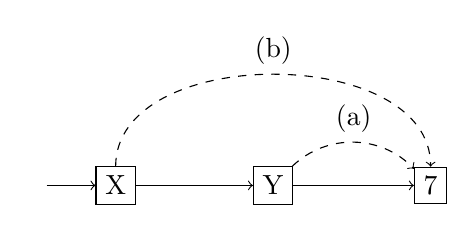
\begin{tikzpicture}[box/.style={draw, rectangle}]
    \node (root) at (-1, 0) {};
    \node[box] (X) at (0, 0) {X};
    \node[box] (Y) at (2, 0) {Y};
    \node[box] (7) at (4, 0) {7};

    \draw[->] (root) -- (X);
    \draw[->] (X) -- (Y);
    \draw[->] (Y) -- (7);

    \draw[->, dashed] (X) to [bend left=90] node [midway, above] {(b)} (7);
    \draw[->, dashed] (Y) to [bend left=45] node [midway, above] {(a)} (7);
\end{tikzpicture}
\caption{Variable shunting during garbage collection. X and Y are shunted variables. Solid lines represent variable bindings. Dashed lines represent the garbage-collection map.}
\label{fig:shunt-cases}
\end{figure}

\end{enumerate}

\subsection{Early Reset}

\label{sec:early-reset}

\emph{Early reset} is concerned with collecting terms that are only accessible from a choice point \cite{applebyGarbargecollectionProlog1988}.

Recall the program in Figure \ref{fig:or-control} (or-control). The first clause of \texttt{run/1} creates a choice point to try the second clause if the first fails, then iterates through an infinite list. As is, the garbage collector is prevented from reclaiming items already iterated over because they are still reachable from the choice point: in the goal \texttt{run(X)}, \texttt{X} is bound to the infinitely-growing list by the execution of the first clause. The key insight behind early reset is that \texttt{X} will be unbound upon backtracking, before the second clause is executed, so it is safe to \emph{reset} (unbind) it ``early'' if it is only reachable from the choice point.

This is implemented during the mark phase. The root set is ordered such that marking from the choice-point stack is done last, so that terms only reachable from the choice-point stack can be identified. When marking each choice point, any currently unmarked variables that will be reset when backtracking to it (i.e. those that are only reachable from the choice-point stack, if at all) are reset.

This introduces a new problem: the entries on the trail stack that have been reset are now garbage themselves. This is resolved by extending the garbage collection algorithm to include a \emph{trail stack compaction} phase, which works analogously to the heap compaction phase.

\subsection{Testing for Precise Garbage Collection}

\label{sec:gc-testing}

Variable shunting and early reset prove sufficient to meet the criteria for precise garbage collection. To test this, for each of the programs in Figure \ref{fig:gc-programs}, I use the following algorithm:

\begin{enumerate}
\item Run the program for a fixed number of iterations to reach a steady state.
\item Perform a garbage collection, then measure the size of the heap.
\item Run the program for a further fixed number of iterations.
\item Perform a garbage collection and measure the size of the heap, passing the test if it is not more than that in step 2.
\item Make one resolution step, then go back to step 4. Repeat this a fixed number of times to get to the same point in the execution as the first measurement, when the test passes.
\end{enumerate}

\subsection{Generational Garbage Collection}

\label{sec:implementation-generational-gc}

While the naive mark-and-sweep garbage collector augmented with variable shunting and early reset is precise, it is not particularly efficient.

Generational garbage collection avoids scanning the entire heap by dividing it into generations, with the youngest generation being collected most frequently (Section \ref{sec:generational-gc}).

\emph{Segmented garbage collection} applies this concept to Prolog \cite{applebyGarbargecollectionProlog1988}. Recall the concept of \emph{age} from the variable shunting algorithm (Section \ref{sec:variable-shunting}). This is used to divide the heap into generations, where each generation consists of a choice point and all terms created since it with no choice points in between. When a choice point (and hence a new generation) is created, terms in previous generations cannot become garbage until the choice point is popped upon backtracking. This means that each garbage collection needs only consider terms in generations for which garbage collection has not yet been performed.

This is implemented by keeping track of the age of the oldest choice point for which garbage collection has not yet been performed. Initially, this is set to 0. When a garbage collection is performed, the age is updated to the size of the heap, which would be the age of a new choice point if one were created immediately. When a choice point is popped, the age is updated to the age of the preceding choice point.

% TODO: say something about trail being write barrier?

\section{JavaScript FFI}

\label{sec:js-ffi}

To better integrate the Prolog interpreter with the web environment, I implemented a foreign function interface (FFI) to enable Prolog code to call JavaScript functions. This section details the implementation of this feature.

\subsection{Augmented Syntax}

I augmented the Prolog syntax with a new term type, \emph{lambda terms}, which represent JavaScript code. A lambda term represents a JavaScript function, along with its arguments, which are Prolog terms. Figure \ref{fig:js-in-prolog} shows an example of a program that delegates to JavaScript to add two numbers.

\begin{figure}[H]
\centering
\begin{minted}{prolog}
add(X, Y, Z) :- <{ (X, Y, Z) => unify(Z, X + Y) }>.
\end{minted}
\caption{Prolog with embedded JavaScript}
\label{fig:js-in-prolog}
\end{figure}

To avoid the LALRPOP-generated parser needing to understand JavaScript syntax, it is extended with a separate recursive descent parser for lambda terms. The LALRPOP grammar identifies strings of tokens enclosed in \texttt{<\{} and \texttt{\}>} as lambda terms, then invokes the recursive descent parser to parse the function into its code and named arguments (Figure \ref{fig:js-grammar}).

\begin{figure}[H]
\centering
\begin{minted}{rust}
LambdaTerm: Term = {
    <js:r"<\{(.|\n)*\}>"> =>? Term::parse_lambda(js)
        .map_err(|error| lalrpop_util::ParseError::User { error }),
}
\end{minted}
\caption{Calling the recursive descent parser in LALRPOP}
\label{fig:js-grammar}
\end{figure}

In Figure \ref{fig:js-in-prolog}, the named arguments are \texttt{X}, \texttt{Y}, and \texttt{Z}, and the JavaScript code is \texttt{unify(Z, X + Y)}, which is evaluated when the lambda term is executed.

\subsection{JavaScript Representation of Prolog Terms}

\label{sec:js-prolog-mapping}

The arguments to such JavaScript functions are Prolog terms, which must be converted to JavaScript objects before the function executes. For ease of JavaScript programming, these are represented using native JavaScript types if possible (e.g. integers as JavaScript numbers). Unbound variables and compound terms are represented using JavaScript objects, the former containing a pointer that is opaque to the JavaScript code (Figure \ref{fig:prolog-js-mapping}).

\begin{figure}[H]
\centering
\begin{subfigure}{0.3\textwidth}
\centering
\begin{minted}{prolog}


a(X, b(3, c))   =>


\end{minted}
\end{subfigure}%
\begin{subfigure}{0.7\textwidth}
\centering
\begin{minted}{javascript}
{ functor: "a",
  args: [
     { variable: (internal pointer) },
     { functor: "b", args: [3, "c"] }
  ] }
\end{minted}
\end{subfigure}
\caption{Representing Prolog terms in JavaScript}
\label{fig:prolog-js-mapping}
\end{figure}

\subsection{Execution of JavaScript}

When the current goal is a lambda term, its JavaScript code is executed:

\begin{enumerate}
\item Rust converts the arguments to JavaScript objects.
\item Rust calls an external JavaScript function called \texttt{eval\_js}, passing it the JavaScript function, serialised arguments, and callback functions for various internal operations (e.g. unification).
\item \texttt{eval\_js} converts the function to a JavaScript \texttt{Function} object, sets up its environment with the callback functions to enable its interaction with WebPL, then calls it with the arguments (Figure \ref{fig:js-execution}).
\end{enumerate}

\begin{figure}[H]
\centering
\begin{minted}{javascript}
try {
    let fn = new Function(...builtin_names, ...arg_names, js)
        .bind(globalThis, ...builtin_values);
    return fn(...arg_values) !== false;
} catch (e) {
    throw e.toString();
}
\end{minted}
\caption{Executing the JavaScript function safely}
\label{fig:js-execution}
\end{figure}

By controlling the environment in which JavaScript code is executed by explicitly providing the internal functions it can call, rather than using \texttt{eval}, the JavaScript code is prevented from corrupting WebPL's state. The functions available to the JavaScript code are detailed in Appendix \ref{appendix:js-ffi}, including \texttt{unify}, which calls back into WebPL to unify two terms.

Alongside returning \texttt{true} on success, the JavaScript function may return \texttt{false} upon logical failure, or throw an exception to indicate an error. In the latter case, the exception is converted to a string before being passed back to Rust.

\section{Web-Based Development Environment}

\label{sec:web-dev-env}

This section describes the implementation of a web-based development environment for WebPL, inspired by the SWISH Prolog IDE \cite{wielemakerSWISHSWIPrologSharing2015}.

\subsection{User Interface}

The user interface (Figure \ref{fig:webpl}) was implemented using the React JavaScript framework. It consists of three main components: the program pane, implemented using \texttt{react-simple-code-editor}, which provides syntax highlighting; the query pane, where the user can enter a query to run against the program; and the results pane, which displays the results of the query.

\begin{figure}[H]
\centering
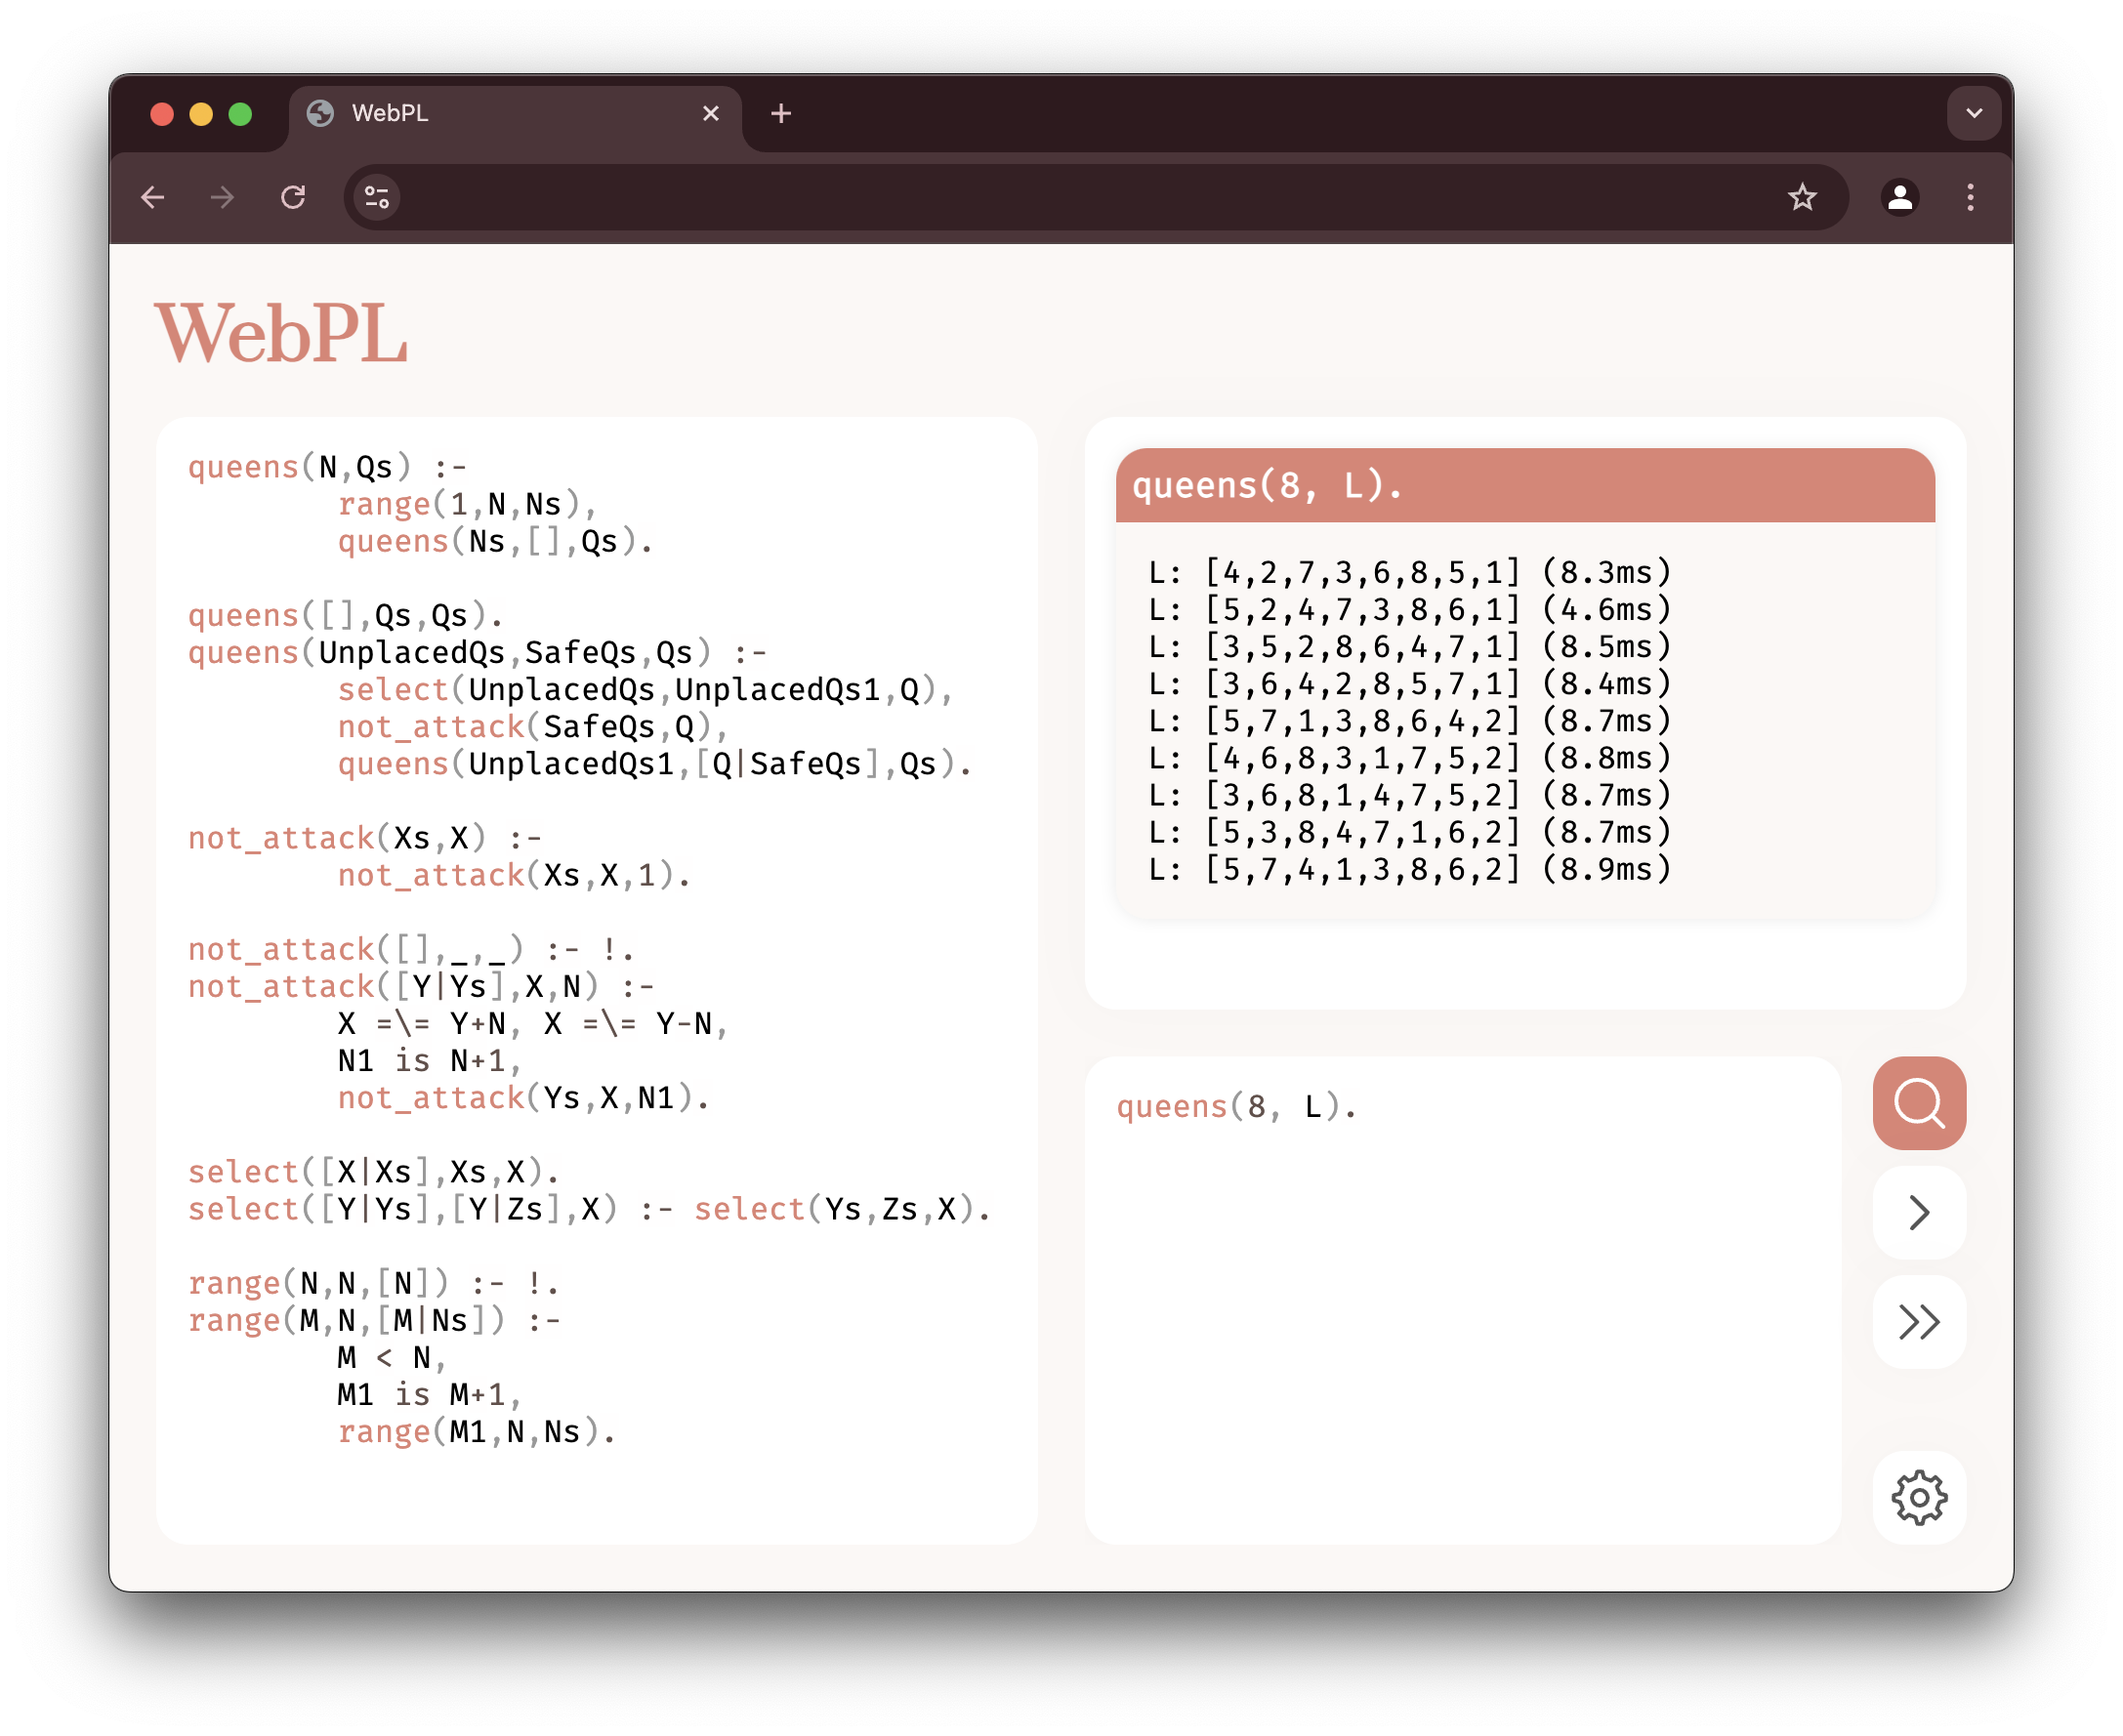
\includegraphics[width=0.85\textwidth]{07implementation_browser.png}
\caption{The web-based development environment running in Chrome on macOS}
\label{fig:webpl}
\end{figure}

\subsection{Prolog Interface}

\label{sec:prolog-interface}

A key goal of the web-based development environment is to support several Prolog implementations to facilitate comparison. Flach et al. highlight the need for a ``standard embedding interface to enable designing interactive web pages using multiple Prolog backends'' \cite{flachSimplyLogicalFirst2023}, which I aim to provide. The TypeScript interface is defined in Figure \ref{fig:prolog-interface}.

\begin{figure}[H]
\centering
\begin{minted}{typescript}
export type Solution = Map<string, string>;
export default abstract class Prolog {
  abstract name: string;
  abstract init(): Promise<void>;
  abstract solve(program: string, query: string): Promise<void>;
  abstract next(): Promise<Solution | undefined>;
  abstract all(): Promise<Solution[]>;
}
\end{minted}
\caption{The Prolog interpreter interface}
\label{fig:prolog-interface}
\end{figure}

\vspace*{-1.5em}

This is an example of the \emph{adapter pattern} \cite{gammaDesignPatternsElements1995}, where an adapter is defined for each Prolog implementation, implementing the \texttt{Prolog} abstract class using the underlying Prolog system. I implemented adapters for WebPL, SWI-Prolog, Tau Prolog, and Trealla Prolog, allowing them to be used interchangeably in the IDE. This abstraction also forms the basis of the benchmarking system (Section \ref{sec:execution-time}).

\subsection{Web Workers}

The programming model in the browser is inherently \emph{asynchronous}, as JavaScript is single-threaded and must not block the main thread to maintain a responsive UI. Long-running computations, like solving a Prolog query, do not fit well into this model, as they block for potentially long periods of time.

Modern browsers provide \emph{Web Workers}, which allow JavaScript to run in a separate thread, communicating with the main thread using an asynchronous message-passing API. Recent Prolog implementations for the browser exploit this feature to prevent Prolog computations from blocking the main thread \cite{garcia-pradalessCASPInBrowserPlayground2022, riazaTauPrologProlog2024}.

\begin{figure}[H]
\centering
\begin{tikzpicture}[
    node distance=1.5cm and 2cm,
    every node/.style={draw, align=center, rounded corners, font=\small},
    every path/.style={<->, thick},
]

\node[draw, thick, minimum width=4cm, minimum height=2.25cm, label=above:{Main Thread}] (main) {};
\node[minimum width=3.5cm, minimum height=0.75cm, below=0.25cm of main.north] (ui) {UI};
\node[minimum width=3.5cm, minimum height=0.75cm, below=0.25cm of ui] (adapter) {Prolog Adapter};
\node[draw, thick, minimum width=4cm, minimum height=2.25cm, right=4cm of main, label=above:{Web Worker}] (worker) {};
\node[minimum width=3.5cm, minimum height=0.75cm, below=0.25cm of worker.north] (engine) {Prolog Engine};
\node[minimum width=3.5cm, minimum height=0.75cm, below=0.25cm of engine] (processor) {Message Processor};

\draw (ui.south) -- (adapter.north);
\draw (adapter.east) -- (processor.west) node[midway, draw=none] {JSON\\message passing};
\draw (processor.north) -- (engine.south);

\end{tikzpicture}
\caption{Web Worker architecture}
\label{fig:web-worker-arch}
\end{figure}

\vspace*{-1.5em}

To use this approach in WebPL, I added configuration options to the adapter for WebPL to run the Prolog interpreter in a Web Worker. When the main thread wants to interact with the Prolog interpreter, the adapter sends a message to the Web Worker, which performs the computation and returns the result to the main thread (Figure \ref{fig:web-worker-arch}). These messages are JSON objects containing the function to call and its arguments.

Since there is no guarantee that messages will be serviced in order, each message is assigned a unique ID which is also present in the response. Before a message is sent, a \texttt{Promise} is created, JavaScript's representation of a pending asynchronous operation. This promise is returned to the caller, and its \emph{resolution} and \emph{rejection} functions are stored in a map, indexed by the message ID. When a response is received, the corresponding function is called with the response or error, allowing success or failure to be handled in JavaScript.